\section{První nastavení}
%%%%%%%%%%%%%%%%%%%%%%%%%%%%
Nastavení celého systému je přístupné skrze systémové nastavení. Do tohoto nastavení má přístup pouze administrátor systému. Přístup do nastavení je vidět na obrázku \ref{fig:Setup_Access}.

\begin{figure}[h!]
    \centering
    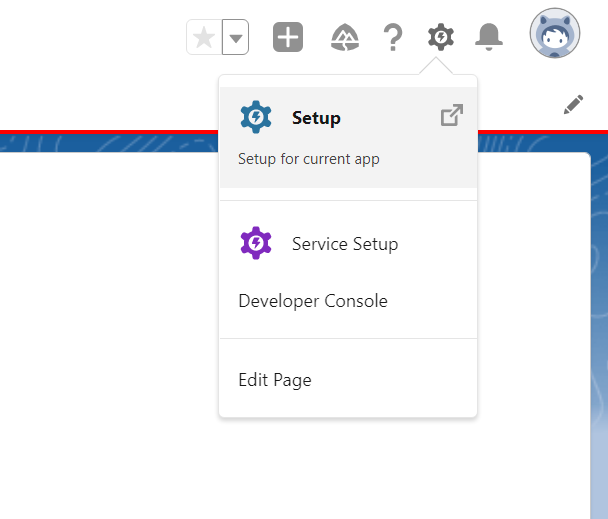
\includegraphics[width=0.65\textwidth]{assets/7_implementace/první_nastavení/Setup.png}
    \caption{Přístup do systémového nastavení.}
    \label{fig:Setup_Access}
\end{figure}

Uživatelské rozhraní v tomto nastavení obsahuje několik důležitých elementů. Na levé straně se nachází menu všech nastavení systému s vyhledávací lištou pro hledání mezi nastaveními. 

V horní části se nachází záložky \emph{Home} a \emph{Object Manager}. Záložka \emph{Object Manager} slouží ke správě objektů. Rozhraní systému je vidět na obrázku \ref{fig:Setup_UI}.

\begin{figure}[h!]
    \centering
    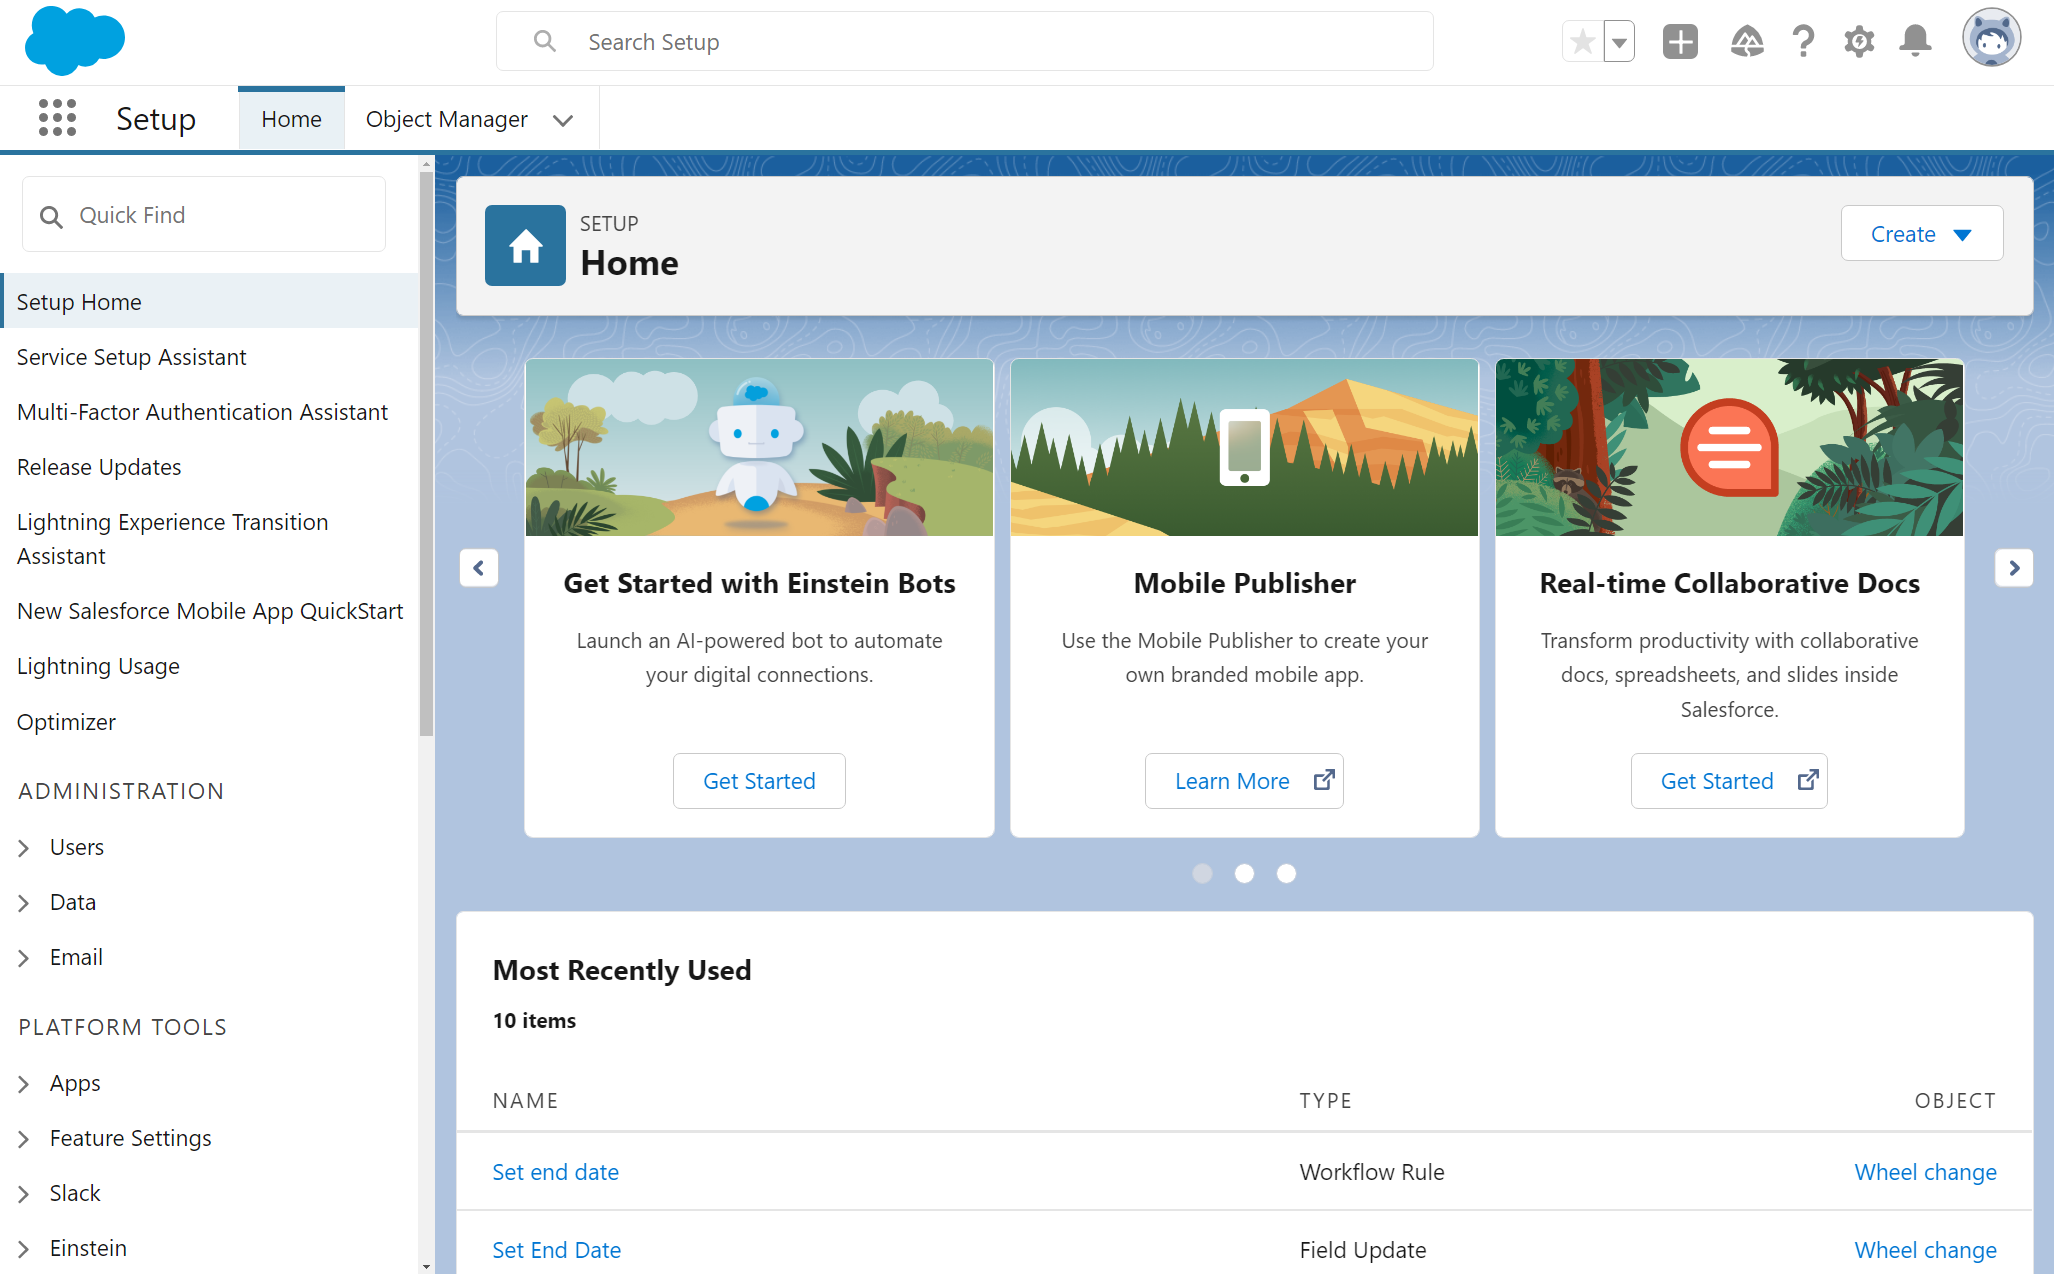
\includegraphics[width=\textwidth]{assets/7_implementace/první_nastavení/setup UI.png}
    \caption{Rozhraní systémového nastavení.}
    \label{fig:Setup_UI}
\end{figure}
\FloatBarrier
